\section{Попередня обробка зображень}

Попередня обробка зображень - перший етап у будь-якій роботі над зображеннями чи відео оскільки у більшості випадків від того, наскільки правильно буде вона проведена, залежить стабільність роботи алгоритмів у подальшому.

Основні причини чому попередня обробка зображень обов'язкова:
\begin{enumerate}
	\item Видалення шумів - випадкові чи невипадкові шуми можуть з'являтися за багатьох причин і дуже сильно впливати на точність роботи системи. Також слід розуміти, що достатньо якісні камери дорого коштують і тому система, яка не буде враховувати випадкові шуми на простих камерах працювати буде погано або навіть кардинально неправильно. До того ж система по локалізації людської руки буде більш затребуваною якщо зможе достатньо добре працювати на простих вебкамерах ноутбуків
	\item Стабілізація форм об'єктів - іноді шуми можуть бути не точкові, а мати деяку форму та спотворювати форму досліджуваних об'єктів на відео. Такі випадки також потрібно враховувати оскільки для видалення таких дефектів використувуються окремі підходи
\end{enumerate}
\subsection{Морфологічні перетворення зображень}
Математична морфологія — це наука, яка вивчає методи і алгоритми аналізу і обробки геометричних структур, основана на теорії множин, топології і випадкових функцій. Застосовується при обробці цифрових зображень, але також може бути застосована до графів, полігональної сітки, стереометрії і бататьох інших просторових структур.

Морфологічні операції виконуються над двома зображеннями: вхідним зображенням і спеціальним, яке залежить від операції і типу виконуваної задачі. Таке спеціальне зображення в математичній морфології називається структурним елементом, примітивом чи ядром. Структурний елемент являє собою деяке двійкове зображення. Він може бути довільного розміру і структури, але за звичай розмір такого зображення має розмір 3x3, 4x4, 5x5 пікселів, тобто значно менше вхідного зображення. Частіше за все використовуються симетричні елементи, такі як прямокутник фіксованого розміру чи круг заданого діаметру. В кожному елементі виділяють особливу точку, яку називають початковою (origin). Вона може вибиратися в будь-якому місці зображення, але найчастіше це центральний піксель.

\begin{figure}[H]
	\centering
	\begin{subfigure}[b]{0.2\textwidth}
		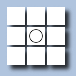
\includegraphics[width=\textwidth]{theory/img/kernel_square}
		\caption{Квадрат}
		\label{fig:kernel_square}
	\end{subfigure}
	\hfill
	\begin{subfigure}[b]{0.2\textwidth}
		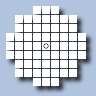
\includegraphics[width=\textwidth]{theory/img/kernel_disk}
		\caption{Диск}
		\label{fig:kernel_disk}
	\end{subfigure}
	\hfill
	\begin{subfigure}[b]{0.2\textwidth}
		
\includegraphics[width=\textwidth]{theory/img/kernel_diamond}
		\caption{Хрест}
		\label{fig:kernel_diamond}
	\end{subfigure}
	\hfill
	\begin{subfigure}[b]{0.2\textwidth}
		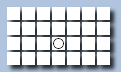
\includegraphics[width=\textwidth]{theory/img/kernel_rectangle}
		\caption{Прямокутник}
		\label{fig:kernel_rectangle}
	\end{subfigure}
	\hfill
	\begin{subfigure}[b]{0.2\textwidth}
		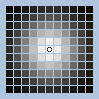
\includegraphics[width=\textwidth]{theory/img/kernel_gauss}
		\caption{Гаусівське ядро}
		\label{fig:kernel_gauss}
	\end{subfigure}
	\caption{Основні структурні елементи}	
\end{figure}

Структурні елементи \ref{fig:kernel_square}, \ref{fig:kernel_disk}, \ref{fig:kernel_diamond} та \ref{fig:kernel_rectangle} складаються лише з 0 та 1. Ядро \ref{fig:kernel_gauss} відрізняється тим, що 1 лише у центрі і далі з віддаленням від центра елементи мають величину, що виражається гаусівським законом розподілу \cite{ErodeDilate}.

Основними морфологічними операціями є:
\begin{enumerate}
	\item Ерозія
	\item Дилація
	\item Розкриття
	\item Закриття
	\item Перенос
\end{enumerate}


\subsubsection{Ерозія}
	\begin{equation}
	A \ominus B = { z \in E | B_{z} \subseteq A}
	\end{equation}
	Інакше кажучи, ерозія множини A по примітиву B, це таке геометричне місце точок для всіх таких позицій точок центру z, при зсуві яких множина B цілком міститься в A.
	
	\begin{figure}[H]
		\centering
		\begin{subfigure}[b]{0.2\textwidth}
			
\includegraphics[width=\textwidth]{theory/img/morph_before}
			\caption{До}
		\end{subfigure}
		\hfill
		\begin{subfigure}[b]{0.2\textwidth}
			
\includegraphics[width=\textwidth]{theory/img/erode_after}
			\caption{Після}
			\label{fig:erode_after}
		\end{subfigure}
		\caption{Ілюстрація операції ерозії}
	\end{figure}

	
\subsubsection{Дилація}
	\begin{equation}
	A \oplus B = { z \in E | B^{\delta}_{z} \cap A \neq \emptyset}
	\end{equation}
	При цьому дилація множини A по структурному елементу B це множина всіх таких переміщень z, при яких множини A і B співпадають принаймні в одному елементі.
	
	\begin{figure}[H]
		\centering
		\begin{subfigure}[b]{0.2\textwidth}
			
\includegraphics[width=\textwidth]{theory/img/morph_before}
			\caption{До}
		\end{subfigure}
		\hfill
		\begin{subfigure}[b]{0.2\textwidth}
			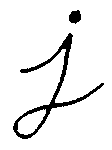
\includegraphics[width=\textwidth]{theory/img/dilate_after}
			\caption{Після}
			\label{fig:dilate_after}
		\end{subfigure}
		\caption{Ілюстрація операції дилації}
	\end{figure}

	
\subsubsection{Розкриття}
	\begin{equation}
	A \circ B = (A \ominus B) \oplus B
	\end{equation}
	Таким чином, розкриття множини A про структурному елементу B знаходиться як ерозія A по B, результат котрої піддається дилації по тому ж структурному елементу B. В загальному випадку розкриття сгладжує контури об’єкту, усуває візькі перешийки і ліквідує виступи невеликої ширини.
	
		
\subsubsection{Закриття}
	\begin{equation}
	A \bullet B = (A \oplus B) \ominus B
	\end{equation}
	
	
	В результаті операції закриття відбувається згладження відрізків контурів, але, на відміну від розкриття, в загальному випадку заповнюються невеликі розриви і довгі заглибини малої ширини, а також ліквідуються невеликі отвори і заповнюються проміжки контуру.
	
\subsubsection{Перенос}
	\begin{equation}
	A_{s} = { a + s | a \in A}, \forall s \in E
	\end{equation}
	Перенос можна визначити за допомогою упорядкованої пари чисел (х,у), де x – кількість пікселів зміщення вздовж осі X, а y – рух вздовж осі Y


\subsection{Видалення шумів шляхом зглажування}

Шуми на цифрових зображеннях доволі поширене явище, особливо якщо зображення було отримане у нестабільних умовах освітлення чи з неякісної камери. Нехтування цим етапом попередньої обробки може призвести до того, що алгоритми також будуть видавати зашумлений результат з великої кількістю дефектів.

Згорткове ядро являє собою матрицю та має деяку особоливу точку в матриці, яку називають центром чи початком. Частіше за все цю точку не задають, а вважають что нею є центр матриці оскільки будь-яке ядро з центром відмінним від центра матриці можна привести до ядра, можливо більшого розміру, щоб його центр співпадав з центром матриці.

Згортка матриці $A$ розмірів $m \times n$ з ядром $K$ розмірів $a \times b$ та центром у точці $(c_{1},c_{2})$ є матриця R, яка будується таким чином:

\begin{equation}
	R_{i,j} = \sum_{x = 1}^{a} \sum_{y = 1}^{b} A_{i-c_{1}+x,j-c_{2}+y}*K_{x,y},
	\:\: i=1..m,j=1..n
	\label{eq:convolution}
\end{equation}

\begin{figure}[H]
	\centering
	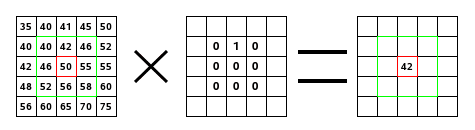
\includegraphics[width=0.7\linewidth]{theory/img/simple_convolution_example}
	\caption{Ілюстрація згортки}
	\label{fig:simple_convolution_example}
\end{figure}

На Рис. \ref{fig:simple_convolution_example} показаний приклад ядра зсуву. Такі ядра називають ядрами зсуву. Вони мають лише одну 1 в матриці, а вектор зсуву можна отримати пободувавши вектор з початком в центрі матриці, а кінцем в одиниці.

Дивлячись на формулу \ref{eq:convolution} можна побачити, що на краях зображення з'являється невизначеність, якої можна позбутися доповнивши матрицю $A$ до розмірів $m+2a \times n + 2b$/.

Доповнювати можна по-різному: нулями, дублювати крайні елементи чи проводити апроксимацію.

Види зглажування выдрізняються лише ядром згортки та операцією над елементами згортки. Як правило операція - сума. Такі фільтри називають лінійними.

\begin{figure}[H]
	\centering
	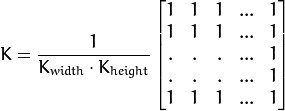
\includegraphics[width=0.7\linewidth]{theory/img/box_filter_representation}
	\caption{Box filter}
	\label{fig:box_filter_representation}
\end{figure}

\begin{equation}
G_{x,y} = Ae^{\frac{-(x-\mu_{x})^{2}}{2\sigma^{2}_{x}} + \frac{-(y-\mu_{y})^{2}}{2\sigma^{2}_{y}}}
\label{eq:gaussian_filter}
\end{equation}

Прикладами лінійних фільтрів є:
\begin{enumerate}
	\item Box filter - прямокутний фільтр. Його ядро має вигляд як на Рис. \ref{fig:box_filter_representation};
	\item Гаусівський фільтр. Елементи матриці мають вигляд щільності двовимірного гаусівскього розподілу \ref{eq:gaussian_filter}.
\end{enumerate}

Прикладами нелінійних фільтрів є:
\begin{enumerate}
	\item Фільтр медіаною - операція над елементами згортки є не сума, а вибір медіани серед них;
	\item Білатеральний фільтр - достатньо потужний фільтр, який дає дуже хороше розмиття зображення, проте він працює значно довше ніж перераховані вище і саме це є його основним недоліком \cite{BilateralFilter}.
\end{enumerate}